\section{Zielsetzung}

Ziel dieses Versuches ist es, das Emmisionsspektrum einer Cu-Röntgenröhre zu untersuchen
sowie die Absorptionsspektren fünf verschiedener Materialien zu analysieren.

\section{Theorie}
\label{sec:Theorie}

\subsection{Röntgenstrahlung}
\label{sec:Röntgenstrahlung}

Für die Erzeugung von Röntgenstrahlung werden in einer evakuierten Röhre aus einer Glühkathode Elektronen emittiert
und zu einer Anode beschleunigt. Beim Auftreffen auf die Anode wird die kinetische Energie der Elektronen in Form von
Röntgenstrahlung abgegeben.

Das Spektrum der Röntgenstrahlung ist in \autoref{fig:Roentgen} zu sehen und setzt sich dabei aus dem
\textit{kontinuierlichen Bremsspektrum} und der \textit{charakteristischen Röntgenstrahlung} zusammen.

\begin{itemize}
    \item Das \textit{kontinuierlichen Bremsspektrum} entsteht aufgrund der Abbremsung der Elektronen,
    da diese ihre kinetische Energie beim Eindringen in das Coulombfeld des Atomkerns in Form von Bremsstrahlung
    abgeben. Es handelt sich um ein kontinuierliches Spektrum, da das Elektron nur eine Teil seiner Energie oder
    im Extremfall die gesamte kinetische Energie abgeben kann.

    \item Die \textit{charakteristischen Röntgenstrahlung} entsteht aufgrund einer Ionisierung des Anodenmaterials.
    Dabei entsteht eine Leerstelle in einer inneren Schale, die von einem Elektron aus einer äußeren aufgefüllt wird.
    Dabei wird ein Röntgenquant emmitiert, dessen Energie genau der Energiedifferenz der Schalen entspricht, also
    \begin{equation*}
        E_{\symup{diff}}=E_{\symup{m}}-E_{\symup{n}}
    \end{equation*}
    Da die Energien der einzelnen Schalen diskret sind, besteht das charakteristische Spektrum aus scharfen Linien, die
    mit $K_{\symup{\alpha}}$, $K_{\symup{\beta}}$, $L_{\symup{\alpha}}$, ... bezeichnet werden. Die Buchstaben $K$, $L$, $M$, ...
    stehen hierbei für die Schalen, auf denen die Übergänge enden. Aus welcher Schale die beteiligten äußeren Elektronen
    kommen, wird durch $\alpha$, $\beta$, $\gamma$, ... angegeben.

    Bei größeren Atomen wird die Kernladung durch die Elektronen abgeschirmt, deshalb wird die Bindungsenergie auf der
    $n$-ten Schale verringert und lässt sich über
    \begin{equation*}
        E_{\symup{n}}=-R_{\infty}z_{\symup{eff}}^{2}\cdot\frac{1}{n^2}
    \end{equation*}
    berechnen. Hierbei ist $R_{\infty}=\qty{13.6}{\electronvolt}$ die Rydbergenergie und $z_{\symup{eff}}=z-\sigma$
    die effektive Kernladung.
    Die Abschirmkonstante $\sigma$ kann empirisch bestimmt werden und wird in \autoref{sec:Abschirmkonstante}
    näher betrachtet.  
\end{itemize}

\begin{figure}[H]
    \centering
    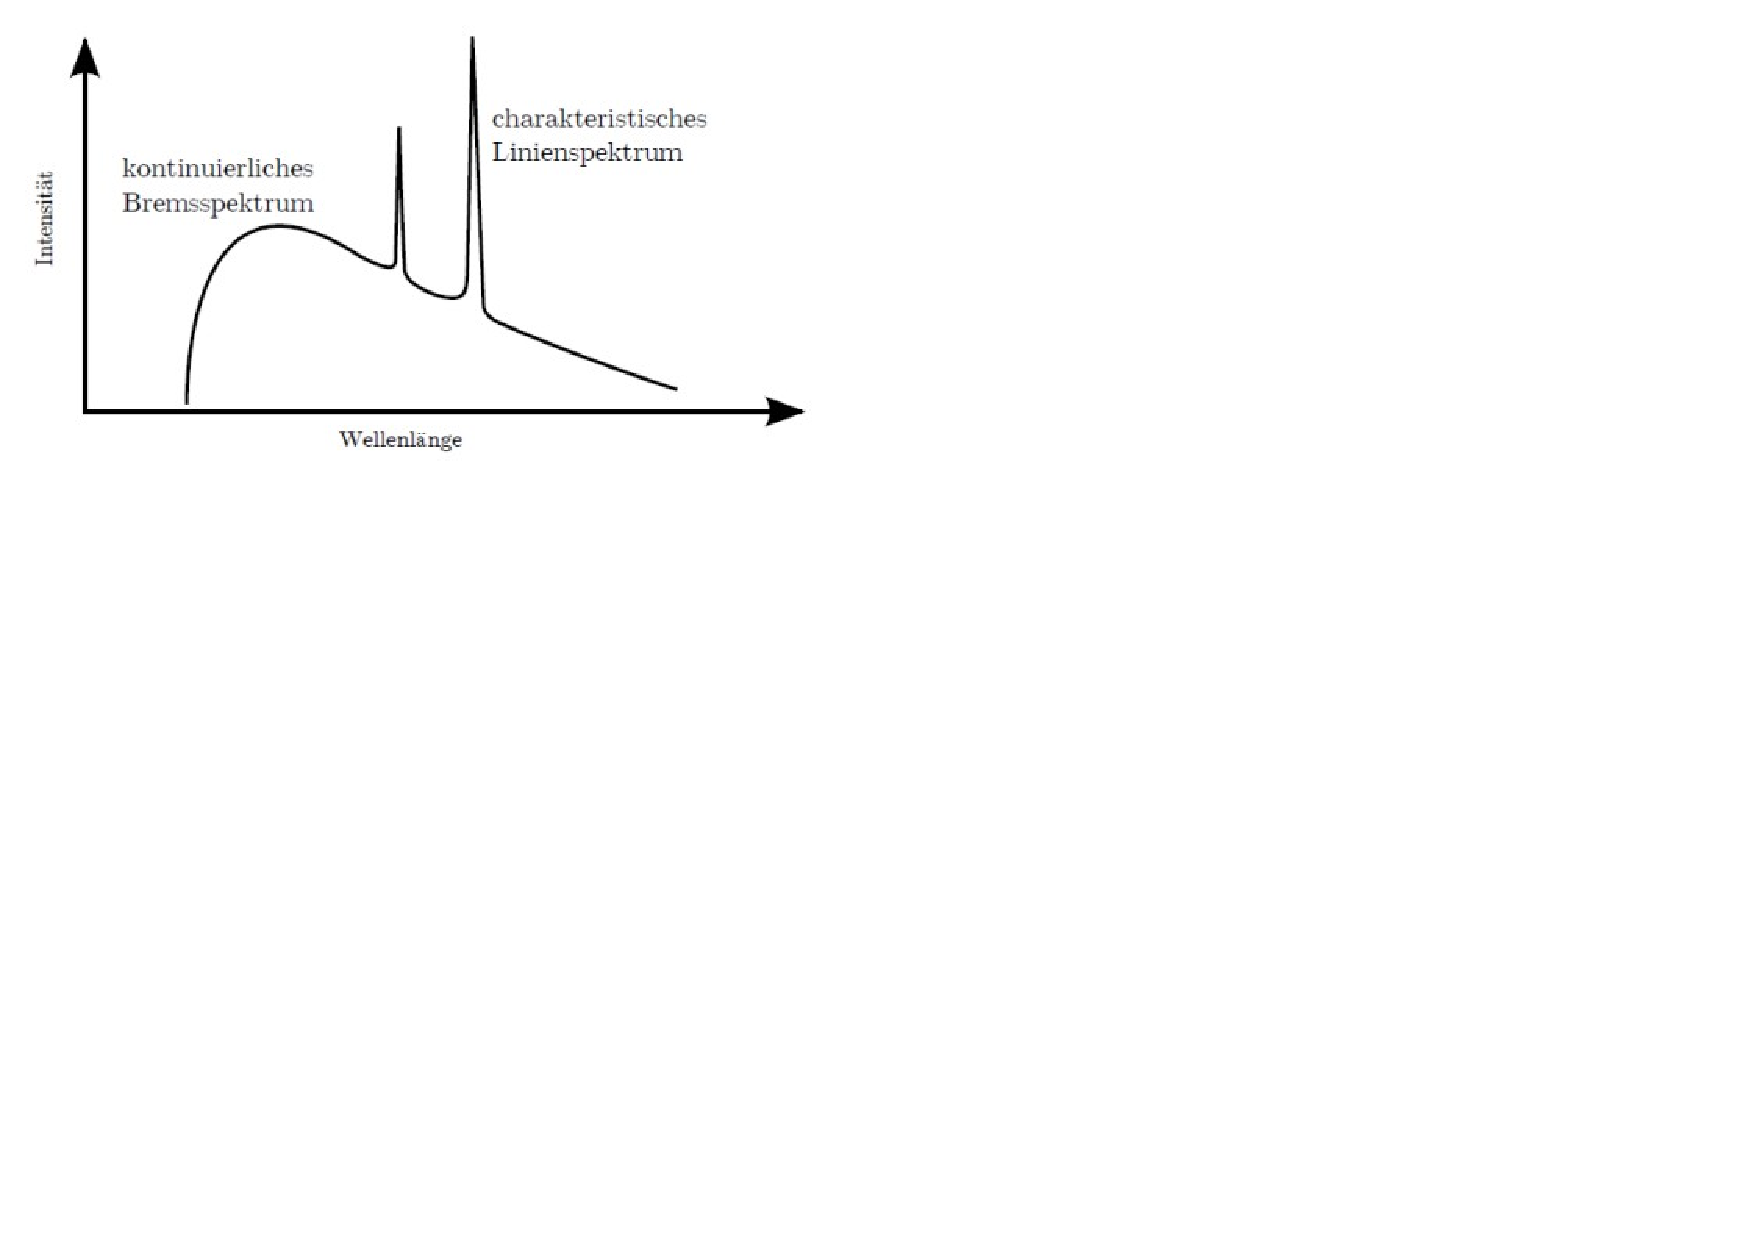
\includegraphics[height=5cm]{content/pics/bremsspektrum.pdf}
    \caption{Qualitative Darstellung des Spektrums von Röntgenstrahlung.\cite{Bremsspektrum}}
    \label{fig:Roentgen}
\end{figure}


\subsection{Absorption von Röntgenstrahlung}
\label{sec:Absorption von Röntgenstrahlung}

Die Absorption von Röntgenstrahlung unter $\qty{1}{\mega\electronvolt}$ findet hauptsächlich durch den Compton- und
Photoeffekt statt, mit zunehmender Energie nimmt die Absorption also ab. Sobald die Energie der Röntgenquanten jedoch
gerade größer ist als die Bindungsenergie eines Elektrons auf der nächsten inneren Schale, steigt die Absorption sprunghaft an,
da der Röntgenquant von einem Elektron aufgenommen werden kann.
Diese Stellen bezeichnet man als Absorptionskanten, sie liegen nahezu an der identischen Stelle wie die Bindungsenergie
des Elektrons. Je nach Schale werden die Bennenung der Kanten mit einem $K$, $L$, $M$, ... versehen, sie sind in
\autoref{fig:Absorption} deutlich zu sehen.

\begin{figure}[H]
    \centering
    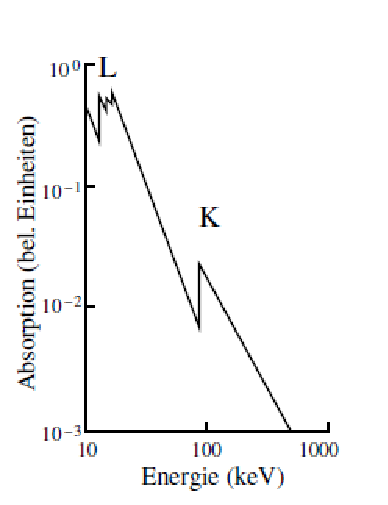
\includegraphics[height=6cm]{content/pics/absorption.pdf}
    \caption{Absorption von Röntgenstrahlung abhängig von der Energie..\cite{v602}}
    \label{fig:Absorption}
\end{figure}

\subsection{Abschirmkonstante}
\label{sec:Abschirmkonstante}

Die zuvor erwähnte Abschirmkonstante wird nun für Kupfer betrachtet.
Da Kupfer vier Schalen besitzt, lassen sich jeweils für die 3 äußeren Schalen die Abschirmkonstanten
$\sigma_1$, $\sigma_2$ und $\sigma_3$ berechnen.

Wenn die Emissionsenergien der $K_{\symup{\alpha}}$- und $K_{\symup{\beta}}$-Linie sowie die Absorptionsenergie
$E_{K\text{, abs}}$ bekannt sind, lassen sich die Abschirmkonstanten über
\begin{align}
    \label{eqn:Sigma_Kupfer}
    E_{K \text{, abs}} &= R_\infty (z - \sigma_1)^2 \\
    \label{eqn:Sigma_Kupfer2}
    E_{K \text{,} \alpha} &= R_\infty \frac{1}{n^2} (z - \sigma_1)^2 - R_\infty \frac{1}{m^2} (z - \sigma_2)^2 \\
    \label{eqn:Sigma_Kupfer3}
    E_{K \text{,} \beta} &= R_\infty \frac{1}{n^2} (z - \sigma_1)^2 - R_\infty \frac{1}{l^2} (z - \sigma_3)^2, 
\end{align}
bestimmen, wobei für Kupfer $n = 1$, $m = 2$ und $l = 3$ gilt.

Eine andere Möglichkeit zur Bestimmung der Abschirmkonstante erfolgt über Betrachtung dees Absorptionsspektrums.
Für die $K$-Schale lässt sich die Abschirmkonstante $\sigma_{\symup{k}}$ über
\begin{equation}
    \label{eqn:sigma_K}
    \sigma_{\symup{k}} = z - \sqrt{\frac{E_{\symup{K}}}{R_\infty} - \frac{\alpha^2 z^4}{4}}
\end{equation}
bestimmen, insofern die Energie der $K$-Kante bekannt ist.
In der Gleichung beschreibt $\alpha$ die Sommerfeldsche Feinstrukturkonstante.

\subsection{Bragg'sche Reflexion}
\label{sec:Bragg'sche Reflexion}

Um die Energie der Röntgenstrahlung zu bestimmen, bietet sich eine Messung der Wellenlänge $\lambda$ an.
Die Energie lässt sich dann leicht über
\begin{equation*}
    E=\frac{hc}{\lambda}
\end{equation*}
bestimmen.
Lässt man Röntgenstrahlung auf ein dreidimensionales Gitter fallen, werden die Photonen an jedem Atom des Gitters gebeugt.
Daher gibt es einen Glanzwinkel $\theta$, bei dem kontruktive Interferenz auftritt, dieser Winkel lässt sich leicht messen.
Diese sognannte Bragg'sche Refelexion ist in \autoref{fig:bragg} dargestellt.
Bei bekannter Gitterkonstante $d$ kann dann die Wellenlänge mithilfe der Bragg'schen Bedingung
\begin{equation}
    2d\sin(\theta)=n\lambda
\end{equation}
berechnet werden.

\begin{figure}[H]
    \centering
    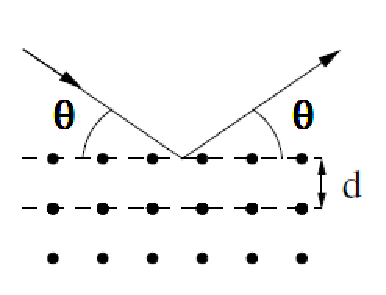
\includegraphics[height=5cm]{content/pics/bragg.pdf}
    \caption{Skizze der Bragg'sche Refelexion.\cite{v602}}
    \label{fig:bragg}
\end{figure}
